\hfill\small{9 Jan 2024}
\vspace{0.5em}
\hrule
\vspace{-0.5em}
\section{Phase Portraits and Limit Cycles}

Consider the system \(\dot{x} = f(x) \) which has an equillibrium point \(x^{\star} \in \mathbb{R}\)
Thus,
\[
    \left . \dot{x}  \right |_{x=x^{\star}} \iff f(x^{\star}) = 0
\]  
\begin{example}[Linear System]
    Consider the case of a linear system given by \(\dot{x} = ax\).
     Then, the equillibrium point is \(x^{\star} = 0\). The solution to the system
     is given by \(x(t) = e^{at} x_0\). The qualitative behaviour of the system 
     depending upon the value of \(a\) is given by the following ``1-D'' phase portrait diagram.

     \begin{center}
        \begin{tikzpicture}
            % Axis lines
            \draw[-] (-2,0) -- (2,0) node[below right] {$x$};
            
            % Arrows pointing towards each other
            \draw[<->] (1,0) -- (-1,0) node[midway]{};
            
            % Origin point
            \draw[] (0,-0.1) -- (0,0.1);
            \node[below right]{$0$};
            \node[right]at (3,0) {$a < 0$};
          \end{tikzpicture}

          \begin{tikzpicture}
            % Axis lines
            \draw[-] (-2,0) -- (2,0) node[below right] {$x$};
            
            % Arrows pointing towards each other
            \draw[>-<] (1,0) -- (-1,0) node[midway]{};
            
            % Origin point
            \draw[] (0,-0.1) -- (0,0.1);
            \node[below right]{$0$};
            \node[right]at (3,0) {$a > 0$};
          \end{tikzpicture}
    \end{center}
    Where the arrows shows the evolution of the trajectory of the system. At \(a = 0\), the
    the entire real line is the equillibria of the system.
\end{example}

\begin{example}[Nonlinear System]
    We will consider a bunch of non linear systems with varying qualitative behaviour.
    \begin{itemize}
        \item \(\dot{x} = x^{2} \quad x \in \mathbb{R} \)
        \begin{center}
            \begin{tikzpicture}
                % Axis lines
                \draw[-] (-2,0) -- (-1,0) node[] {};
                \draw[-] (1,0) -- (2,0) node[below right] {$x$};
                
                % Arrows pointing towards each other
                \draw[<-<] (1,0) -- (-1,0) node[midway]{};
                
                % Origin point
                \draw[] (0,-0.1) -- (0,0.1);
                \node[below right]{$0$};
              \end{tikzpicture}
        \end{center}
        \item \(\dot{x} = x^{2} - 1 \quad x \in \mathbb{R}\) 
        \begin{center}
            \begin{tikzpicture}
                % Axis lines
                \draw[-] (-3,0) -- (-2,0) node[] {};
                \draw[>-<] (-2,0) -- (0,0) node[] {};
                \draw[->] (0,0) -- (2,0) node[] {};
                \draw[-] (2,0) -- (3,0) node[below right] {$x$};
                
                
                \draw[] (-1,-0.1) -- (-1,0.1);
                \node [below right] at (-1,0) {$-1$};
                \draw[] (1,-0.1) -- (1,0.1);
                \node [below right] at (1,0) {$1$};
              \end{tikzpicture}
        \end{center}
        \item \(\dot{x} = 1\quad x \in \mathbb{R}\)
        \begin{center}
            \begin{tikzpicture}
                % Axis lines
                \draw[-] (0,0) -- (2,0) node[below right] {$x$};
                
                % Arrows pointing towards each other
                \draw[->] (-2,0) -- (0,0) node[midway]{};
              \end{tikzpicture}
        \end{center}
        \item \(\dot{x} = \sin (x) \quad x \in \mathbb{R}\)
        \begin{center}
            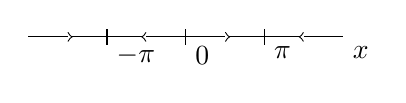
\begin{tikzpicture}
                % Axis lines
                \draw[-] (1.5,0) -- (2,0) node[below right] {$x$};
                % Arrows pointing towards each other
                \draw[>-<] (0.5,0) -- (1.5,0) node[midway]{};
                \draw[-] (-0.5,0) -- (0.5,0) node[midway]{};
                \draw[>-<] (-1.5,0) -- (-0.5,0) node[midway]{};
                \draw[-] (-2,0) -- (-1.5,0) node[midway]{};
                \draw[] (-1,-0.1) -- (-1,0.1);
                \draw[] (1,-0.1) -- (1,0.1);
                \draw[] (0,-0.1) -- (0,0.1);
                \node [below right] at (0,0) {$0$};
                \node [below right] at (1,0) {$\pi$};
                \node [below right] at (-1,0) {$-\pi$};
              \end{tikzpicture}
        \end{center}
    \end{itemize}
    
\end{example}

\subsection{2D Phase Portraits}
Let the two dimensional system be defined by
\[
    \dot{x}_1 = f_1(x_1, x_2) \quad \dot{x}_2 = f_2(x_1, x_2) \implies \dot{x} = f(x)  
\]
The phase portrait in some rough sense can be thought of as the ``trajectory'' of the system,
and where we care about the slope of the vector field of \(f(x)\) is given by:
\[
    \frac{\dot{x}_2}{\dot{x}_1} = \frac{f_2(x)}{f_1(x)}  
\] 
The phase portrait of the linear system can be easily understood via the jordan normal form
of the system.

Consider the system given by, \(\dot{x} = Ax \), and the linear transformation given by \(y = Px\),
Thus we get,
\[
    \dot{y} = P\dot{x} = PAx = PAP^{-1}y = Jy  
\]  
where \(J\) is the jordan normal form of \(A\).

We can have one of the 3 cases of the jordan form. The forms with their characteristic
polynomials are given by:

\[
    \begin{aligned}
        J_1 &= \begin{bmatrix}
            \lambda_1  &  0 \\
            0 &  \lambda _2 \\
        \end{bmatrix} \implies  p(s) = (s-\lambda _1) (s-\lambda _2)\\
        J_2 &= \begin{bmatrix}
            \lambda_1  &  1 \\
            0 &  \lambda _1 \\
        \end{bmatrix} \implies  p(s) = (s-\lambda _1) ^2\\
        J_3 &= \begin{bmatrix}
            \alpha  &  -\beta  \\
            \beta  &  \alpha  \\
        \end{bmatrix} \implies  p(s) = (s-\alpha) ^2 + \beta ^2\\
    \end{aligned}
\]
The solution of the equation in the transformed coordinates is given by:
\[
    y(t) = e^{Jt} y(0) \implies  x(t) = P ^{-1} e^{Jt} P x(0)
\]
Thus, the solution can be split into three cases similar to the one done above\\
\textbf{Case 1:}
\[
    y_1(t) = e^{\lambda _1 t} y_1(0) \quad y_2(t) = e^{\lambda _2 t} y_2(0)
\]
Thus, depending on the value of \(\lambda _1\) and \(\lambda _2\), we can have the following
phase portraits:\\
\medskip%
\begin{minipage}
    {0.5\textwidth}
    \input{figures/phaseportraits/case11.tex}
\end{minipage}
\begin{minipage}
    {0.5\textwidth}
    \begin{center}
    \begin{tikzpicture}[
        declare function={f(\x,\y) = 3 * \x ;},
        declare function={g(\x,\y) = 1 * \y ;}
        ]
        \begin{axis}[
            simplePhase,
            title={$\lambda_1<\lambda _2<0$},
            width=\textwidth
          ]
          \addplot3 (x,y,0);
        \end{axis}
      \end{tikzpicture}
\end{center}
\end{minipage}
\centerline{\begin{minipage}
    {0.5\textwidth}
    \begin{center}
    \begin{tikzpicture}[
        declare function={f(\x,\y) = 1 * \x ;},
        declare function={g(\x,\y) = 1 * \y ;}
        ]
        \begin{axis}[
            simplePhase,
            title={$\lambda_1<\lambda _2<0$},
            width=\linewidth
          ]
          \addplot3 (x,y,0);
        \end{axis}
      \end{tikzpicture}
    \end{center}
\end{minipage}}\\
% \begin{center}
    \begin{tikzpicture}[
        declare function={f(\x,\y) = 1 * \x ;},
        declare function={g(\x,\y) = 1 * \y ;}
        ]
        \begin{axis}[
            simplePhase,
            title={$\lambda_1<\lambda _2<0$},
            width=\linewidth
          ]
          \addplot3 (x,y,0);
        \end{axis}
      \end{tikzpicture}
    \end{center}

% \input{figures/phaseportraits/case11.tex}
% \begin{center}
    \begin{tikzpicture}[
        declare function={f(\x,\y) = 3 * \x ;},
        declare function={g(\x,\y) = 1 * \y ;}
        ]
        \begin{axis}[
            simplePhase,
            title={$\lambda_1<\lambda _2<0$},
            width=\textwidth
          ]
          \addplot3 (x,y,0);
        \end{axis}
      \end{tikzpicture}
\end{center}
\medskip
\textbf{Case 2:}
\[
    \begin{aligned}
        y_1(t) &= e^{\lambda t} \left(   y_1(0) + t y_2(0)  \right)\\
        y_2(t) &= e^{\lambda t} y_2(0)
    \end{aligned}
\]
Simillary, we can have the following phase portraits depending on the value of \(\lambda\):\\
\medskip%
\begin{minipage}
    {0.5\textwidth}
    \begin{center}
    \begin{tikzpicture}[
        declare function={f(\x,\y) = -2 * \x + \y ;},
        declare function={g(\x,\y) = -2 * \y ;}
        ]
        \begin{axis}[
            simplePhase,
            title={$\lambda < 0$: Improper Stable Node},
            width=\textwidth
          ]
          \addplot3 (x,y,0);
          \addplot +[magenta] {0.5 * x};
        \end{axis}
      \end{tikzpicture}
    \end{center}
    
\end{minipage}
\begin{minipage}
    {0.5\textwidth}
    \input{figures/phaseportraits/case22.tex}
\end{minipage}\\
\medskip%
\textbf{Case 3:} Let \( r\coloneqq \sqrt{y_1 ^{2} + y_{2^{2} }  } \) and \(\theta \coloneqq \tan ^{-1}  \left( \frac{y_2}{y_1}  \right) \)
Substituing the values of \(y_1\) and \(y_2\) in the equation, and simplifying, we get:
\[
    \dot{r} = \alpha r \quad \dot{\theta} = \beta 
\]
Thus, switching in the polar form, the transformed system are evolving independently of each other.
The phase portrait is given by:\\
\medskip%
\begin{minipage}
    {0.5\textwidth}
    \input{figures/phaseportraits/case31.tex}
\end{minipage}
\begin{minipage}
    {0.5\textwidth}
    \begin{center}
    \begin{tikzpicture}[
        declare function={f(\x,\y) = 2 * \x - \y ;},
        declare function={g(\x,\y) = \x + 2 * \y ;}
        ]
        \begin{axis}[
            simplePhase,
            title={$\lambda < 0$: Unstable Focus},
            width=\textwidth
          ]
          \addplot3 (x,y,0);
        \end{axis}
      \end{tikzpicture}
    \end{center}
    
\end{minipage}\\
%%%%%%%%%%%%%%%%%%%%%%%%%%%%%%%%%%%%%%%%%%%%%%%%%%%%%%%%%%%%%%%%%

\subsection{Linearization}

Consider a non linear system \(\dot{x} = f(x)\) with an equillibrium point \(x^{\star} = 0\).
Then using first order Taylor series expansion, we have:
\[
    \dot{x} = f(x) = f(0) + \left . \frac{\partial f}{\partial x} \right |_{x=0} x + \mathcal{O}(x^2)
\]

Thus, the linearised system can be written as:
\[
    \dot{x} = A x \quad \text{where} \quad A = \left . \frac{\partial f}{\partial x} \right |_{x=0}
\]
The matrix \(A\) is called the \emph{Jacobian} of the system \(\dot{x} = f(x)\) evaluated at the
equillibrium point \(x^{\star} = 0\). The system can also be calculated for an equillibrium point
not at origin, by shifting the origin to the equillibrium point.
    
\subsubsection{Pertubations of the eigenvalues}
The study of the behaviour of linear systems about the equillibrium point \(x=0\) is important
beacuse in many cases the behaviour of a nonlinear systems, near an equillibrium point can
be deduced by linearsing the system about the equillibrium point.

The validity and the accuracy of the linearization of the nonlinear system, and the resultant
qualitative behaviour depends on the placement of the eigenvalues of the linearised system.
This can be understood by considering the linear pertubations. Let the linearized system be
given by \(\dot{x} = Ax, x\in\mathbb{R} \), with distinct eigenvalues, and let
\(\Delta A \in \mathbb{R}^{2\times 2}\) be a small pertubation matrix, whose elements have arbitrary
small magnitudes. We know, that the eigenvalues of the matrix \(A + \Delta A\)
depend continuously on the parameters of the matrix. 

Thus, when the matrix \(A\) is pertubed by \(\Delta A\), any eigenvalues of A that lies in
the left or the right half plane, wil remain in its respective half plane. But, the eigenvalues
on the imaginary axis, when perturbed might go into either the left or the right half plane.

Consquently, we can say that if the equillibrium point \(x=0\) of \(\dot{x} = Ax \) is a
node, focus, or saddle, then the equillibrium point \(x=0\) of \(\dot{x} = (A + \Delta A) x \)
will be of the same type, provided that the pertubations are small enough. This situation is quite different in the case of center. Since the qualitative behaviour of the
stable focus and unstable focus are different from that of a center, the center equillibrium 
point will not persist under pertubations.

The node, focus, and saddle equillibrium point are said to be \emph{structurally stable} because they
maintain their qualitative behaviour under infinitesimally small pertubations.

\begin{definition}[Hyperbolic Equillibrium Point]
    An equillibrium point of the system \(\dot{x}= f(x)\) with \(f(x^{\star}) = 0\) is said to be
    hyperbolic if:
    \[
        \Re \left(
            A = \left . \frac{\partial f}{\partial x} \right |_{x=x^{\star}}
        \right) \neq 0
    \] 
    i.e. the jacobian of the system evaluated at the equillibrium point has no eigenvalues
    with zero real part.
\end{definition}

\begin{example}
    Consider the system \(\dot{x} = x^3 , x\in\mathbb{R} \)
    The system has its only equillibrium point at \(x^{\star} =0\). The phase portrait of the system
    is given by:
    \begin{center}
        \begin{tikzpicture}
            % Axis lines
            \draw[-] (-2,0) -- (2,0) node[below right] {$x$};
            
            % Arrows pointing towards each other
            \draw[<->] (1,0) -- (-1,0) node[midway]{};
            
            % Origin point
            \draw[] (0,-0.1) -- (0,0.1);
            \node[below right]{$0$};
        \end{tikzpicture}
    \end{center}
    linearsing the system we have \(\dot{x} = 3x^2 \implies \dot{x} = 0 \).
    
    Thus we can say that for any arbitrary point close to the equillibrium point, the behaviour
    described by the linear system is different from the non linear system
\end{example} 
\begin{example}
    Consider the system given by:
    \[
        \begin{aligned}
            \dot{x}_1 &= -x_2 -\mu x_1 (x_1^2 + x_2^2)\\
            \dot{x}_2 &= x_1 - \mu x_2 (x_1^2 + x_2^2)
        \end{aligned}
    \]
    The system has an equillibrium point at \(x^{\star} = 0\).
    Linearsing the system around the origin we have:
    \[
        A = \left . \frac{\partial f}{\partial x} \right |_{x=0} = \begin{bmatrix}
            0 & -1 \\
            1 & 0
        \end{bmatrix} \implies \lambda = \pm i
    \]
    Note that the linearised system corresponds to a simple harmoic oscillator
    
    Shifting, into polar coordinates to analyse the system, we have:
    \[
        r\coloneqq \sqrt{x_1^2 + x_2^2} \quad \theta \coloneqq \arctan \left( \frac{x_2}{x_1} \right)
    \]
    After some simplification, we have:
    \[
        \dot{r} = -\mu r^3 \quad \dot{\theta} = 1 
    \]
    Depending upon the value of \(\mu\), we have the following:
    \[
        \begin{aligned}
            \mu > 0 &\implies \text{Stable Focus} \\
            \mu = 0 &\implies \text{Center} \\
            \mu < 0 &\implies \text{unstable Focus} \\
        \end{aligned}  
    \]
    Thus, the qualitative behaviour is same for the linearised system and the nonlinear system,
    only at \(\mu = 0\), which can also be trivally observed from the state equations.
\end{example}
Thus, we have a sufficient condition for the qualitative behaviour of the nonlinear system to be
same as the linearised system, which is that the equillibrium point of the nonlinear system should
be hyperbolic.

\begin{theorem}[Hartman-Grobman Theorem]
Let \(\dot{x}=f(x),\:x\in\mathbb{R}^n\) be a nonlinear system with an hyperbolic
equillibrium point \(x_e\). Let \(\phi_t^f\) be the flow map for \(\dot{x}=f(x)\) i.e. \(\dot{x}=f(x),\:x(0)=x_0\)
has the solution \(x(t)=\phi_t^f(x_0)\). Then for a \(\delta >0\) and a ball \(B_{\delta}(x\in\mathbb{R}^n \vert
\Vert x-x^{\star}\Vert < \delta)\) there exits as map \(F : B_{\delta} \subset \mathbb{R}^n \to \mathbb{R}^n, \: \exists T > 0\)
such that, 
\[
    F(x_e) = 0, \text{ F is one to one on } B_\delta \text{ onto } F(B_\delta)  
\]        
and both \(F\) and \(F^{-1} \) exits and are continuous, such that \(F(\phi_t^f) = e^{At}F(x) \quad \forall \vert t \vert
< T\). Where \(A = \left . \frac{\partial f}{\partial x} \right |_{x=x^{\star}}\) and \(x\in B_\delta \)\\

\begin{tikzpicture}
    \node[label=below:$x_0$]  (x0) at (-0.1,1)  {$\bullet$};
    \node[label=below:$x(t)$]  (xt) at (0.5,2)  {$\bullet$};
    \node[label=below:$F(x_0)$]  (Fx) at (6,1)  {$\bullet$};
    \node[label=right:$e^{At}F(x_0)$]  (eAF) at (9,4)  {$\bullet$};
    \draw (0,1.5) circle (1.0) ;
    \node[label=left:$x_e$]  (xe) at (-0.75,1.45)  {$\bullet$};
    \draw (x0.center) to [out=5,in=-90]++(0.25,1.1) to[out=15,in=-95](xt.center); %% in the ball
    % \draw (Fx.center) to [out=10,in=-110]++(2.6,2) to[out=70,in=-103](eAF.center); %%
    \draw (Fx.center) to [out=15,in=-105](eAF.center);
    \begin{scope}[dashed,decoration={
        markings,
        mark=at position 0.5 with {\arrow{>}}}
        ] 
    \draw[postaction={decorate}] (x0.center) to [out=10,in=-520](Fx.center); %%
    \draw[postaction={decorate}] (xt.center) to [out=10,in=-150](eAF.center); %%
    \draw[postaction={decorate}] (eAF.center) to [out=150,in=10](xt.center); %%
    \node at (3,0.25) {$F$};
    \node at (4.75,2.25) {$F$};
    \node at (4.5,3.25) {$F^{-1} $};eAF.center
    \end{scope}
\end{tikzpicture}
\label{thm:hartmanGrobman}
\end{theorem}
\vspace{0.5em}

The map \(F\) in \autoref{thm:hartmanGrobman} maps from the nonlinear world to the linear world. 
\subsubsection{Pendulumn}
One example of periodicity in phase portraits is given by the pendulumn. 
This type of periodic behaviour is not found in linear systems.
\begin{example}[Pendulumn]
    Consider a pendulumn, with normalised dynamics given by:
    \[
        \begin{aligned}
            \dot{x}_1 &= x_2  \\
            \dot{x}_2 &= -\sin(x_1) - x_2
        \end{aligned}
    \]
    The equillibrium points of this system are given by:
    \[
        x_1 = k\pi \quad x_2 = 0 \quad k\in\mathbb{Z}
    \]
    Calculating the jacobian of the system, we have:
    \[
        A = \left . \frac{\partial f}{\partial x} \right |_{x=x^{\star}} = \begin{bmatrix}
            0 & 1 \\
            -\cos(x_1) & -1
        \end{bmatrix}
    \]
    Evalating the jacobian at \((0,0)\) and \((\pi,0)\) we have :
    \[
        \begin{aligned}
            \left. \frac{\partial f}{\partial x} \right |_{x=(0,0)} &= \begin{bmatrix}
                0 & 1 \\
                -1 & -1
            \end{bmatrix} \implies \lambda = \frac{-1 \pm \sqrt{3}}{2} \\
            \left. \frac{\partial f}{\partial x} \right |_{x=(\pi,0)} &= \begin{bmatrix}
                0 & 1 \\
                1 & -1
            \end{bmatrix} \implies \lambda = \frac{-1 \pm \sqrt{5}}{2} \\
        \end{aligned}
    \]
    The phase portrait of the system is given by:
    \begin{center}
        \includegraphics[width=\linewidth]{figures/phaseportraits/pend.png}
    \end{center}
    The image source is \href{https://tikz.net/dynamics_phaseportrait/}{linked here}
\end{example}
%%%%%%%%%%%%%%%%%%%%%%%%%%%%%%%%%%%%%%%%%%%%%%%%%%%%%%%5

\subsection{Limit Cycles and Periodic Orbits}

Periodic orbits in the phase plane, which have a closed trajectory is usually 
called a perioidc orbit or closed orbit. An isolated perioidc orbit is called as a limit cycle.

For examples a harmonic oscillator has there is a continuum of cloed orbits as 
shown in the \autoref{fig:harmonic-oscillator}
, while in the case 
of Van der Pol oscillator, there is only one closed orbit i.e. a limit cycle as shown in
\autoref{fig:van-der-pol-oscillator}.

\begin{minipage}
    {0.5\textwidth}
    \begin{figure}[H]
        \centering
        \includegraphics[width=0.9\textwidth]{figures/phaseportraits/osc.png}
        \caption{Harmonic Oscillator}
        \label{fig:harmonic-oscillator}
    \end{figure}
\end{minipage}
\begin{minipage}
    {0.5\textwidth}
    \begin{figure}[H]
        \centering
        \includegraphics[width=0.9\textwidth]{figures/phaseportraits/van.png}
        \caption{Limit Cycle in Vander Pol Oscillator}
        \label{fig:van-der-pol-oscillator}
    \end{figure}
\end{minipage}

\subsection{Poincar\'e-Bendixson Theorem and Bendixson's Criterion}
Periodic orbits divide the plane into a region inside the orbit and a region outside it.
This allows us to obtains criteria for the existence of periodic orbits in a region of the plane.
The analysis of such a kind doesn;t extend to higher dimensions, as there is no concept of
inside and outside in higher dimensions. One such criteria is given by the Poincar\'e-Bendixson
theorem.

\begin{theorem}[Poincar\'e-Bendixson Theorem]
Let \(\dot{x} = f(x) , x \in \mathbb{R}^2\) and there exists a closed and bounded set
\(M \subset \mathbb{R}^2\) such that:
\begin{itemize}
    \item \(M\) contains no equillibrium points of \(\dot{x} = f(x)\)
    \item Every trajectory that starts in \(M\) remains in \(M\) for all \(t \geq 0\) 
\end{itemize} 
Then \(M\) contains a periodic orbit of \(\dot{x} = f(x)\).
\end{theorem}

\subsubsection*{Math Review:}
\[
    \Div f = \text{ divergence of vector field } f
\]
\[
    \Div f = \sum_{i=1}^{n} \frac{\partial f_i}{\partial x_i} \quad \text{where } f = (f_1, f_2, \dots, f_n)
\]
For a 2D vector field F we have:
\[
    \Div F = \frac{\partial f_1}{\partial x_1} + \frac{\partial f_2}{\partial x_2} \quad x \in \mathbb{R}^2
\]
If there are no sources or sinks in a region (which are equillibrium points in context 
of dynamical systems), then the divergence of the vector field is zero.

\begin{theorem}[Divergence and Green's Theorem]
    THe divergence theorem states that the volume integral of the divergence of a vector field
    is equal to the surface integral of the vector field over the boundary of the volume. i.e.
    \[
        \iiint{V} \Div F dV = \iint_{S} F \cdot n dS
    \]
    where \(n\) is the outward normal to the surface \(S\).

   Green's theorem states that the line integral of a vector field over a closed curve is equal
    to the surface integral of the curl of the vector field over the region bounded by the curve.
    i.e.
    \[
        \oint_{C} F \cdot dr = \iint_{S} \curl F \cdot n dS
    \]
    \[
        \implies \iint_S \left( 
            \frac{\partial f_1}{\partial x_1} + \frac{\partial f_2}{\partial x_2}
         \right) dS = \oint f_2(x_1, x_2) dx_1 - f_1(x_1, x_2) dx_2
    \]
\end{theorem}

Thus, we can now state teh Bendixson's criterion as follows:
\begin{theorem}[Bendixson's Criterion]
    Let \(D\) be a simply connected region in \(\mathbb{R}^2\). Suppose 
    \(f\) is such that \(\Div f = \dfrac{\partial f_1}{\partial x_1} + \dfrac{\partial f_2}
    {\partial x_2}\) is not identically zero in \(D\), and doesn't change sign in \(D\).
    Then there are no periodic orbits of \(\dot{x} = f(x)\) entirely in \(D\).
\end{theorem}
\begin{proof}
    Proof by contradiction: Suppose there exists a perioidc orbit \(\gamma \) that in 
    entirly in \(D\), for any trajectory of \(\dot{x} = f(x) \quad x \in \mathbb{R} ^{2} \)
    
    \[
        \frac{\mathrm{d}x_2}{\mathrm{d}x_1} = \frac{f_2 (x)}{f_1 (x)} \implies 
         f_2 (x) \mathrm{d}x_2 - f_1 (x) \mathrm{d}x_1 = 0
    \]
    \[
        \implies \oint_{\gamma} f_2 (x) \mathrm{d}x_2 - f_1 (x) \mathrm{d}x_1 = 0
    \]

    By Green's theorem, we have:
    \[
        \iint_S \left( 
            \frac{\partial f_1}{\partial x_1} + \frac{\partial f_2}{\partial x_2}
         \right) = 0
    \]

    This contradictcs the fact the divergence of \(f\) is not identically zero in \(D\), thus
    volating our assumption. Hence Proved.
\end{proof}

\subsection{Index of a curve}
\begin{definition}[Index of a curve]
    For a sufficiently smooth vector field \(f: \mathbb{R} ^{2} \to \mathbb{R} ^{2} \) and a 
    closed curve \(\gamma \) not passing through any equillibrium points of \(\dot{x} = f(x)\), the
    index of \(\gamma\) w.r.t.\ \(f\) is:
    \[
        I^f_\gamma = \frac{1}{2\pi} \oint_{\gamma} d\theta_f \qquad \theta = \tan^{-1} \left( 
            \frac{f_2}{f_1}
         \right)
    \]
\end{definition}
\vspace{1em}
There are certain properties of the index of a curve listed below:
\begin{property}[1]
    If we have two closed curves \(\gamma_1\) and \(\gamma_2\) such that \(\gamma_1\)
    can be continuously deformed into \(\gamma_2\) without passing through any equillibrium
    points then,
    \[
        I^f_{\gamma_1} = I^f_{\gamma_2}
    \]
\end{property}
\begin{property}[2]
    If \(\gamma \) doesn not enclose any equillibrium points, then
    \[
        I^f_{\gamma} = 0
    \] 
\end{property}
\begin{property}[3]
    \[
        I^f_\gamma = I^{-f}_\gamma 
    \]
    This can be intituitively understood as follows:
    \[
        \theta _f = \pi + \theta _{-f} \implies d\theta _f = - d\theta _{-f}
    \]
    Thus equating the line integral
\end{property}
\begin{property}[4]
    If \(\gamma \) is a closed orbit of \(\dot{x} = f(x)\) then
    \[
        I^f_\gamma = 1
    \]
\end{property}
\begin{property}[5]
    If \(\gamma \) encloses one equillibrium point \(x^*\), and \(x^{\star} \) is
    a hyperbolic equillibrium point, then:
    \[
        A = \left. \frac{\partial f}{\partial x} \right|_{x^{\star}} \implies 
        I^f_\gamma = I^{Ax}_\gamma 
    \] 
\end{property}

Using the above properties, we can now define the index of the equillibrium point.

\begin{definition}[Index of an equillibrium point]
\(I(x^{\star} _i)\) is the index of the equillibrium point \(x^{\star} _i\) of \(\dot{x} = f(x)\)
where \(I(x^{\star} _i)\) is the index of any closed curve \(\gamma \) enclosing only
\(x^{\star} _i\) and no other equillibrium points.  
\end{definition}
\begin{lemma}
    Index of a node, focus or a center is \(1\), while that of a saddle is \(-1\).
\end{lemma}
\begin{lemma}
    Index of a closed curve is the sum of the indices of the equillibrium points enclosed
    by the curve \(\gamma \)
\end{lemma}

Thus, we have the following corollary:

\begin{corollary}
    Inside any perioidc orbit \(\gamma \) there exists at least one equillibrium point. Suppose
    all the equillibrium points inside \(\gamma \) are hyperbolic. Let \(N\) be the number of
    nodes, foci and centers inside \(\gamma \) and \(S\) be the number of saddles inside \(\gamma \).
    then, the index of \(\gamma \) is:
    \[
        I^f_\gamma = N - S
    \] 
\end{corollary}


